\documentclass[fleqn]{article}
\usepackage[english]{babel}
\usepackage{a4wide}
\usepackage{latexsym}
\usepackage{times}
\usepackage{theorem}
\usepackage{url}
\usepackage[final]{graphics}
\usepackage{amsmath,amssymb}
\usepackage{amsfonts}
\usepackage{array}
\usepackage{calc}
\usepackage{xspace}
\usepackage{color}
\usepackage{epsfig}
\usepackage{subfigure}
\usepackage{float}
\usepackage{stmaryrd}
\usepackage{color}
\usepackage{mathtools}
\usepackage{graphicx}
\usepackage{epstopdf}
\usepackage{listings}
\usepackage{color}
\usepackage{booktabs,caption}
%\usepackage[flushleft]{threeparttable}
\usepackage{amsmath}


\DeclareMathAlphabet{\mathpzc}{OT1}{pzc}{m}{it}

\usepackage{amssymb}
\usepackage{graphicx}
\usepackage{epstopdf}
\usepackage{mathtools}

\usepackage{algorithm}
\usepackage[noend]{algpseudocode}

\usepackage{fouriernc}
\pagestyle{plain}
\usepackage{float}
\usepackage[hidelinks]{hyperref}

\usepackage{array}
\newcolumntype{L}[1]{>{\raggedright\let\newline\\\arraybackslash\hspace{0pt}}m{#1}}
\newcolumntype{C}[1]{>{\centering\let\newline\\\arraybackslash\hspace{0pt}}m{#1}}
\newcolumntype{R}[1]{>{\raggedleft\let\newline\\\arraybackslash\hspace{0pt}}m{#1}}

\newtheorem{theorem}{Theorem}
\newtheorem{fact}{Fact}
\newtheorem{hypothesis}{Hypothesis}
\newtheorem{lemma}{Lemma}
\newtheorem{definition}{Definition}

\definecolor{codegreen}{rgb}{0,0.6,0}
\definecolor{codegray}{rgb}{0.5,0.5,0.5}
\definecolor{codepurple}{rgb}{0.58,0,0.82}
\definecolor{backcolour}{rgb}{0.95,0.95,0.92}

\lstdefinestyle{mystyle}{
	backgroundcolor=\color{backcolour},   
	commentstyle=\color{codegreen},
	keywordstyle=\color{magenta},
	numberstyle=\tiny\color{codegray},
	stringstyle=\color{codepurple},
	basicstyle=\footnotesize,
	breakatwhitespace=false,         
	breaklines=true,                 
	captionpos=b,                    
	keepspaces=true,                 
	numbers=left,                    
	numbersep=5pt,                  
	showspaces=false,                
	showstringspaces=false,
	showtabs=false,                  
	tabsize=2
}

\lstset{style=mystyle}


\usepackage{fouriernc}
\pagestyle{plain}

%% macros.tex

\title{\sf Hold time lower bound}
\author{{\sf H.J. Rivera Verduzco 0977393}\\
{\footnotesize\sl P.O.~Box 513, 5600 MB Eindhoven, The Netherlands}\\
{\footnotesize \sl Email: \tt H.J.Rivera.Verduzco@student.tue.nl}}
%\date{}
\begin{document}
\maketitle

%\begin{abstract}
%\noindent
% Add abstract here %
%\end{abstract}

\section{BCHT for FPTS}

Given a task-set $\mathpzc{T}$, Algorithm 1 shows a procedure to derive a less pessimistic lower bound for the \textit{best-case hold time} of a task $\tau_i$. Table \ref{tab:terminology} explain the terminology for the variables used in the algorithm. Furthermore, function $BI_i(y,PA_d)$ returns the the largest positive solution satisfying

\begin{align}
x = y + \sum\limits_{h:\pi_h > \theta_i} \Big( \Big\lceil  \dfrac{x}{T_h}\Big\rceil -1 \Big)^+  BC_h + \sum\limits_{d:\theta_i \geq \pi_d \pi_i} \Big( \Big\lceil  \dfrac{x-PA_d}{T_d}\Big\rceil -1 \Big)^+  BC_d,
\end{align}

\noindent
where the notion $w^+$ stands for $\max(w,0)$.

\begin{table}[H]
	\center
	\caption{Terminology.}
	\label{tab:terminology_ht}
	\begin{tabular}{|c | p{9cm}|}
		\hline
		Name & Descriptions \\ 
		\hline 
		\hline
		$HLB^{init}_i$& Initial lower bound. This is the \textit{best-case hold time} of task $\tau_i$ when considering only preemptive tasks.\\
		\hline
		$BH^{lb}_i$& Lower bound of the \textit{best-case hold time} of $\tau_i$; $BH_i \geq BH^{lb}_i.$\\
		\hline
		$UB_i$& Upper bound in hold time when pushing the activation of delaying tasks. \\ 
		\hline
		$PI_i$ & Push interval of delaying tasks relative to $BH^{lb}_i$.   \\ 
		\hline
		$DI_i$ & Delay interval of task $\tau_i$ is the time interval in which delaying tasks can affect the hold time.\\
		\hline 
	\end{tabular}
	%\small
	%\item The \textit{least common multiple} of the periods is 240 and $U^{\mathpzc{T_{\ref{tab:taskset2}}}} \approx 0.96$.
\end{table} 

\begin{algorithm}[H]
	\caption{Algorithm to derive a tighter lower bound for the \textit{best-case hold time} of task $\tau_i$.}\label{euclid}
	\begin{algorithmic}[1]
		\Procedure{\textit{bchtLowerBound}}{$\mathpzc{T},i$}
		\State $HLB^{init}_i = BI_i(BC_i,\infty)$;
		\State $BH^{lb}_i = HLB^{init}_i$;
		\State $UB_i = BI_i(BC_i,BH^{lb}_i)$;
		\While {$UB_i > HLB^{init}_i$}
		\State $DI_i = UB_i - BH^{lb}_i$;
		\State $PI_i = \min \limits_{d:\theta_i \geq \pi_d > \pi_i} (DI_i \mod T_d);$
		\State $BH^{lb}_i = BH^{lb}_i + PI_i$;
		\State $UB_i = BI_i(BC_i,BH^{lb}_i)$;
		\EndWhile{\textbf{end while}}
		\State \Return $BH^{lb}_i$; 
		\EndProcedure
	\end{algorithmic}
\end{algorithm}

%\begin{algorithm}[H]
%	\caption{Algorithm to derive a tighter lower bound for the \textit{best-case hold time} of task $\tau_i$.}\label{euclid}
%	\begin{algorithmic}[1]
%		\Procedure{\textit{HLB}$_i$}{$\mathpzc{T}$}
%		\State $HLB^{init}_i = BI_i(BC_i,\infty)$;
%		\State $PI_i = -\delta$;
%		\State $LB_i = HLB^{init}_i + PI_i$;
%		\State $UB_i = BI_i(BC_i,LB_i)$;
%		\If {$UB_i > HLB^{init}_i$}
%		\State $LB_i = HLB^{init}_i$;
%		\EndIf {\textbf{end if}}
%		\While {$UB_i > HLB^{init}_i$}
%		\State $DI_i = UB_i - LB_i$;
%		\State $PI_i = \min \limits_{d:\theta_i \geq \pi_d > \pi_i} (DI_i \mod T_d);$
%		\State $LB_i = LB_i + PI_i$;
%		\State $UB_i = BI_i(BC_i,LB_i)$;
%		\EndWhile{\textbf{end while}}
%		\State \Return $LB_i$; 
%		\EndProcedure
%	\end{algorithmic}
%\end{algorithm}

In order to illustrate how the algorithm works, consider the task-set $\mathpzc{T}_{\ref{tab:taskset5}}$ described in Table \ref{tab:taskset5}. Figure \ref{fig:bcht_1} shows the notions after performing Algorithm 1 to calculate $BH^{lb}_4=55$. Note that in Figure \ref{fig:bcht_1}, the second job of $\tau_3$ activated at time $t=30$, namely $\iota_{3,2}$, does not start. This is to illustrate that the \textit{best-case hold time} of $\tau_4$ should be long enough in order to delay the start time of $\iota_{3,2}$, i.e. $BH_4 > BH^{lb}_4$. If this condition is not met, the job $\iota_{3,2}$ will start and delay the start time of $\tau_4$. As a consequence, the job of $\tau_4$ will experience preemptions by the higher priority tasks activated at time $t=85$.

\begin{table}[H]
	\center
	\caption{Task set $\mathpzc{T}_{\ref{tab:taskset5}}$.}
	\label{tab:taskset5}
	\begin{tabular}{c c c c c | c c c c}
		\hline 
		& $T_i$ & $WC_i=BC_i$ & $\pi_i$ & $\theta_i$ &  $wl_i$ & $BR_i$ & $BH^{lb}_i$ & $HLB^{init}_i$\\ 
		\hline 
		$\tau_1$& 80  & 14  & 4 & 4 &  1 & 14 & &\\
		$\tau_2$& 80  & 6   & 3 & 3 &  1 & 6  & &\\ 
		$\tau_3$& 30  & 15  & 2 & 2 &   & 15  & &\\ 
		$\tau_4$& 240 & 50  & 1 & 2 &   & 56  & 55& 50\\
		\hline 
	\end{tabular}
	\small
	\item The \textit{least common multiple} of the periods is 240 and $U^{\mathpzc{T_{\ref{tab:taskset5}}}} \approx 0.96$.
\end{table}

\begin{figure}[H]
	\centering
	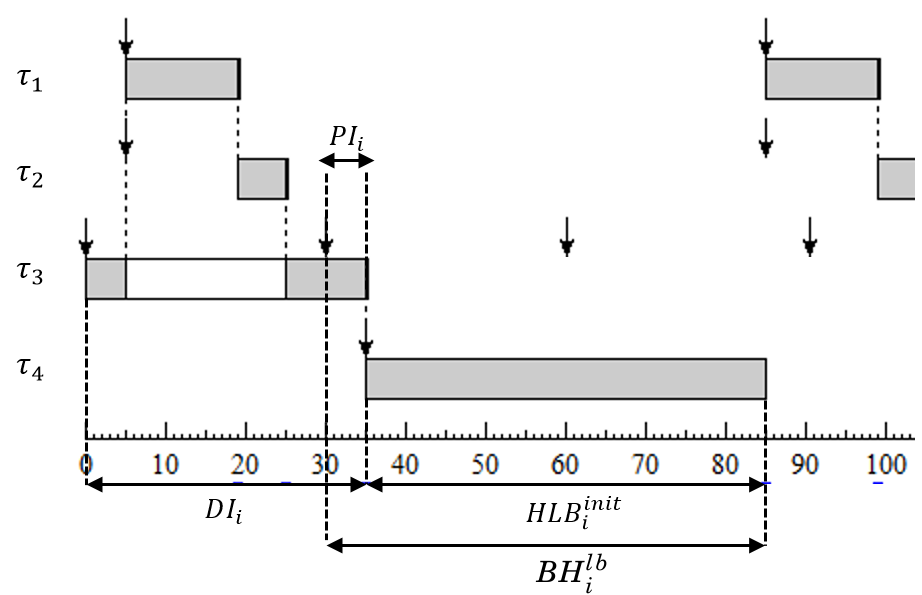
\includegraphics[width=0.7\linewidth]{figures/bcht_1}
	\caption{Schedule of task-set $\mathpzc{T}_{\ref{tab:taskset5}}$ with the notions described in Table \ref{tab:terminology}.}
	\label{fig:bcht_1}
\end{figure}

Note that the only way for the job of task $\tau_4$ to have a hold time higher than $BH^{lb}_4=55$ is by experiencing preemption by either task $\tau_1$, $\tau_2$ or both. Since $\tau_2$ has a \textit{best-case execution time} $BC_2=6$, we can choose this task to preempt $\tau_4$ and the condition will be met because $HLB^{init}_4+BC_2= 56$ which is higher than $BH^{lb}_4 = 55$. This is indeed the \textit{best-case hold time} because if we would choose $\tau_1$ to preempt $\tau_4$, the resulting hold time would be $HLB^{init}_4+BC_1= 64$. Figure \ref{fig:bcht_2} shows the schedule where the \textit{best-case hold time} of task $\tau_4$ is assumed.

\begin{figure}[H]
	\centering
	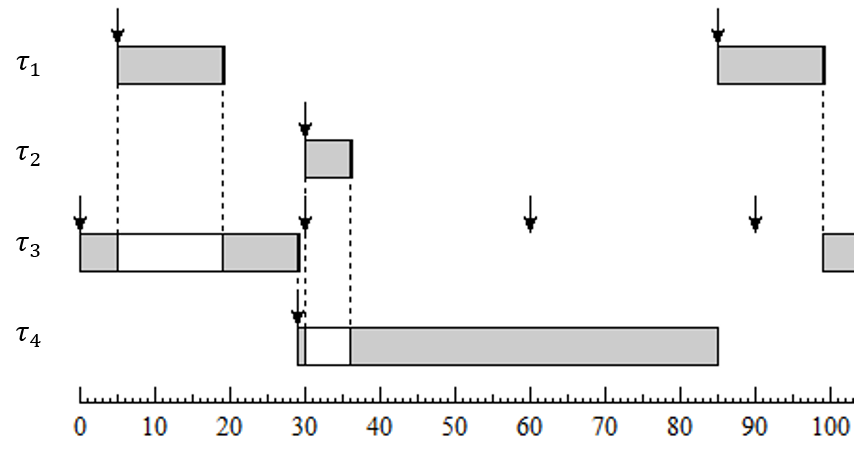
\includegraphics[width=0.7\linewidth]{figures/bcht_2}
	\caption{Schedule of task-set $\mathpzc{T}_{\ref{tab:taskset5}}$ where the \textit{best-case hold time} of task $\tau_4$ is assumed ($BH_4 = 56$).}
	\label{fig:bcht_2}
\end{figure}



\begin{thebibliography}{10}


	
\end{thebibliography}


\end{document}

